\section{目的}

依講義 PDF 第 85--87 頁比較動態 DFF 的直接時脈、兩級反相器時脈回復與三級暫存器 skew，並觀察低頻保持。

\section{講義要求與對應測試}

\begin{center}
\small
\setlength{\tabcolsep}{4pt}
\begin{tabular}{p{.42\linewidth}p{.29\linewidth}p{.18\linewidth}}
\toprule
要求 & 網表編號與條件 & 狀態 \\
\midrule
步驟 1：放慢時脈邊緣並提高頻率 & 01; direct, 9 pairs & 已量測 \\
步驟 2：加入兩級反相器後重做 & 01; buffered, same pairs & 已量測 \\
步驟 3：三級 DFF、第三時脈超前/落後 & 02; 9 signed skews & 已量測 \\
固定輸入時脈 rise/fall 0.2 ns & 02; fixed source slew & 已保留 \\
問題 1：低頻儲存；問題 2/3：buffer/race & 03; 10 us, 25/115 C & 量測與分析 \\
\bottomrule
\end{tabular}
\end{center}

\section{電路與時序推導}

直接版以理想互補電壓產生兩相；buffer 版取兩級反相器第一級與第二級輸出作互補相位，因此包含真實延遲、非完全同時的轉換及額外負載。三級鏈中前兩級共用同一組 buffered clock，第三級由獨立延遲的原始脈衝經相同兩級 inverter 產生。正 skew 定義為第三級 clock 落後。

以目的端 clock 落後量 $s$ 表示，常用約束為 $t_{CQ,\max}+t_{PD,\max}+t_{SU}\leq T+s$ 與 $t_{CQ,\min}+t_{CD,\min}\geq t_H+s$。正 skew 可能放寬 setup、卻加重 hold；所以 buffer 能回復斜率，不保證消除 race。

\section{模擬設定與判讀方式}

以提供的加密 MOS 模型、1.0 V 供應、25\,$^\circ$C 為基準。1.0 V 是教學測試條件，並非已核實的額定電壓；沒有把本次結果當作講義原製程或原供應電壓的重現。除網表另註，$W_n/W_p/L=0.6/1.8/0.25\,\mu\mathrm m$，Bulk 接對應電源軌，輸出負載為 5 fF。傳輸閘與弱回授器件的例外尺寸均在網表明列。

使用 PrimeSim HSPICE S-2021.09 win64、\texttt{RUNLVL=6}、\texttt{ACCURATE} 及 \texttt{WARNLIMIT=100}。每份網表的主分析與 \texttt{.alter} 均完成，沒有 error 或 failed measurement；但模擬器仍回報加密區塊的警告被隱藏，因此不能宣稱模型無警告或警告無害。\texttt{.tran} 的列印間隔不是固定積分步長；求解器使用自適應步長。本次沒有把有限的掃描範圍當作完整製程認證。

除非另註，功能診斷以低電位 $V\leq0.2$ V、高電位 $V\geq0.8$ V 判定；這是本報告公開採用的判讀規則，不是講義給定的數值門檻，也不是已萃取的接收器雜訊容限。取樣正確不能排除取樣間毛刺。所有圖均由實際輸出資料重繪；\texttt{results/} 保存逐案例波形、量測與衍生比較 CSV。

公開網表不含模型載入路徑；模擬時在本機副本加入模型設定，模型本體不在交付資料內。網表檔名的前兩位數對應下表編號，各檔可獨立執行。

\section{結果}

\begin{center}
\small
\setlength{\tabcolsep}{4pt}
\begin{tabular}{lrrr}
\toprule
週期 (ns) & 斜率 (ns) & 直接正確/8 & buffer 正確/8 \\
\midrule
20 & 0.2 & 8 & 8 \\
20 & 1 & 8 & 8 \\
20 & 5 & 8 & 8 \\
10 & 0.2 & 8 & 8 \\
10 & 1 & 8 & 8 \\
10 & 2 & 8 & 8 \\
4 & 0.2 & 8 & 8 \\
4 & 1 & 4 & 4 \\
2 & 0.2 & 8 & 4 \\
\bottomrule
\end{tabular}
\end{center}

取樣在每週期 $0.49T$，相對原始 clock 上升開始 $0.25T$；buffer 的延遲會消耗同一觀察期限。4 ns/1 ns 的兩版均僅 4/8 正確；2 ns/0.2 ns 直接版 8/8、buffer 版 4/8。因此不能根據這張表聲稱 buffer 一定提高內部最高頻率。需分開看邊緣品質、插入延遲與接收端的實際取樣時間。

\begin{figure}[htbp]
\centering
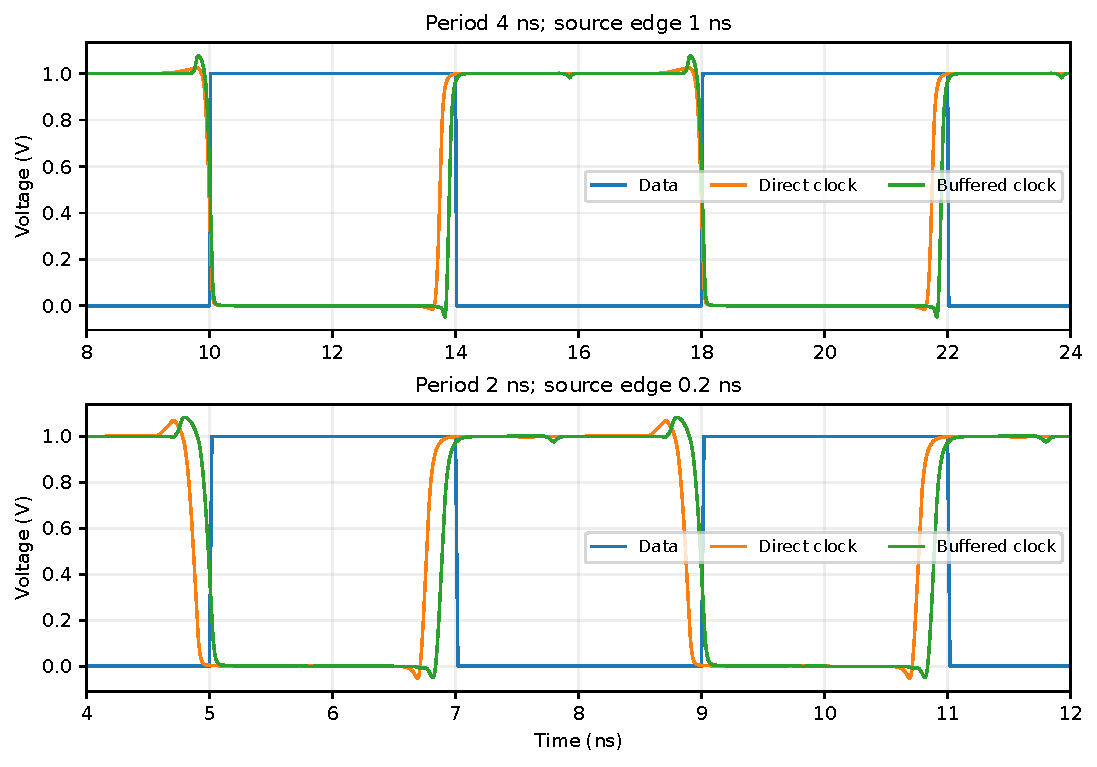
\includegraphics[width=.96\linewidth]{figures/clock_slope.pdf}
\caption{兩個接近觀察期限的案例；buffer 的延遲會影響固定時間判讀。}
\end{figure}

\begin{center}
\small
\setlength{\tabcolsep}{4pt}
\begin{tabular}{lrrr}
\toprule
第三時脈 skew (ns) & 正確樣本/7 & 第一樣本 (V) & 第二樣本 (V) \\
\midrule
0 & 7 & 1.00001 & 0.00000 \\
-0.2 & 7 & 1.00001 & 0.00000 \\
-0.5 & 7 & 1.00001 & 0.00000 \\
-1 & 7 & 1.00001 & 0.00000 \\
-2 & 7 & 1.00001 & 0.00000 \\
0.2 & 7 & 1.00001 & 0.00000 \\
0.5 & 0 & 0.00000 & 1.00000 \\
1 & 0 & 0.00001 & 1.00001 \\
2 & 0 & 0.00000 & 1.00000 \\
\bottomrule
\end{tabular}
\end{center}

0 至 +0.2 ns 落後仍為 7/7；+0.5 ns 起變成相反資料序列而為 0/7，符合目的端過晚造成同週期資料穿透的 hold/race 現象。-0.2 到 -2 ns 超前的已測點均為 7/7，不能外推成任意負 skew 都安全。這裡的邊界只被 +0.2 與 +0.5 ns 夾住，未做連續二分萃取。

\begin{figure}[htbp]
\centering
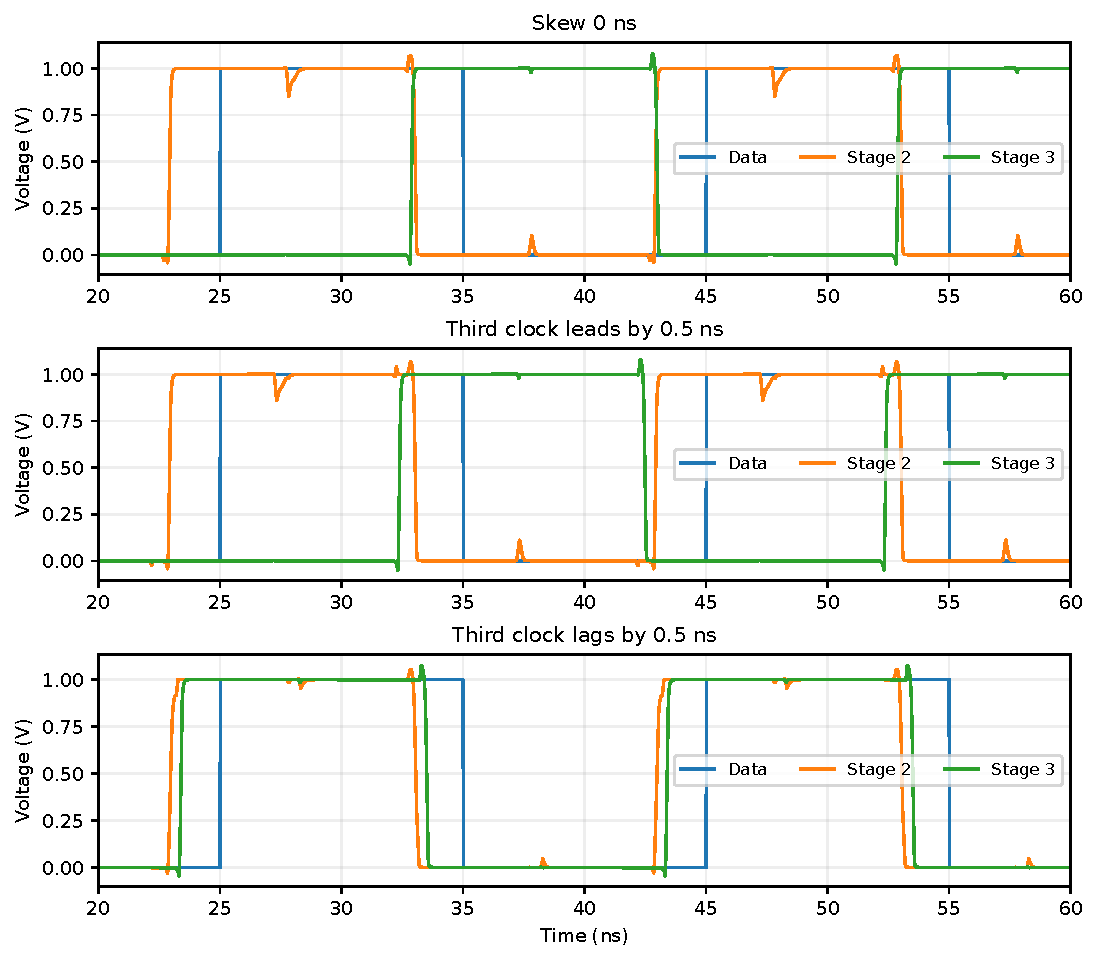
\includegraphics[width=.96\linewidth]{figures/clock_skew.pdf}
\caption{三級鏈在零 skew、第三級超前及落後時的資料序列。}
\end{figure}

\begin{center}
\small
\setlength{\tabcolsep}{4pt}
\begin{tabular}{lrr}
\toprule
溫度 (C) & master X，7 us (V) & slave Z，12 us (V) \\
\midrule
25 & 0.582685 & 0.084038 \\
115 & 0.662096 & 0.117369 \\
\bottomrule
\end{tabular}
\end{center}

\begin{figure}[htbp]
\centering
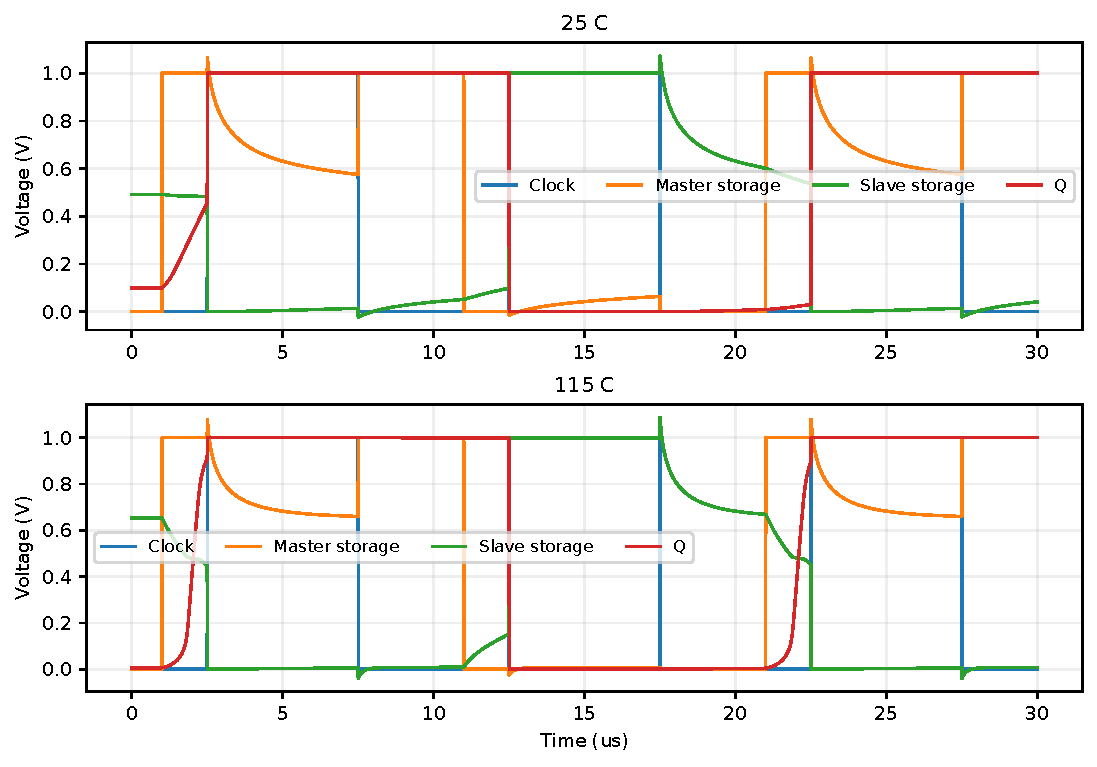
\includegraphics[width=.96\linewidth]{figures/slow_clock.pdf}
\caption{10 us 週期下的內部浮接儲存節點。}
\end{figure}

\section{討論、差異與尚未證實的範圍}

低頻時浮接節點偏離電源軌，即使選定時刻的輸出仍可能正確，也已不能把動態 latch 當作無限期儲存。兩個溫度的淨漏電結果不是單一接面漏電萃取，不能強加所有節點皆隨溫度單調惡化。改善方案包括靜態/弱回授保持、非重疊兩相、控制 clock tree skew 與滿足 setup/hold；NORA/TSPC 可改變 race 條件，但仍受類比耦合與資料時序限制。原檔只作參考，本重寫補齊同條件 direct/buffer 比較、雙方向 skew 與低頻內部節點，並把兩級時脈 buffer 的實際延遲納入解釋。
